\documentclass{icga}
\newif\iflong\longfalse  %change to longtrue for longer version
% additional long version material like this:
% \iflong
% ... long version material ...
% \fi

\usepackage{url}
\usepackage{graphicx}
\def\Eo{\mbox{\sc Ezo}}
\def\Hite{\mbox{\sc Hexcited}}
\def\Hent{\mbox{\sc Hexcellent}}
\def\Mx{\mbox{\sc MoHex}}
\def\Mc{\mbox{\sc MoHex-CNN}}
\def\Sol{\mbox{\sc Solver}}
\def\Fuego{\mbox{\sc Fuego}}

\title{\sc MOHEX WINS HEX 11x11 AND 13x13 TOURNAMENTS}
\runningtitle{ICGA}
\author{Ryan Hayward\thanks{Department of Computing Science, 
University of Alberta, Canada. Email:hayward@ualberta.ca},
Noah Weninger \thanks{CS, UAlberta, Email:nweninge@ualberta.ca}
}
\affiliation{Edmonton, Canada}
\issue{to appear in ICGA Journal}

\setcounter{page}{999}
\begin{document}
\maketitle

%\iflong
%In the longer version of the report, we include all games.
%\fi

\vspace*{-2.25in}
%{\it ICGA Journal Report Computer Games Olympiad, 2017 Leiden.}
{\it to appear, ICGA Journal}
\vspace*{2.0in}

\begin{figure}[hbt]
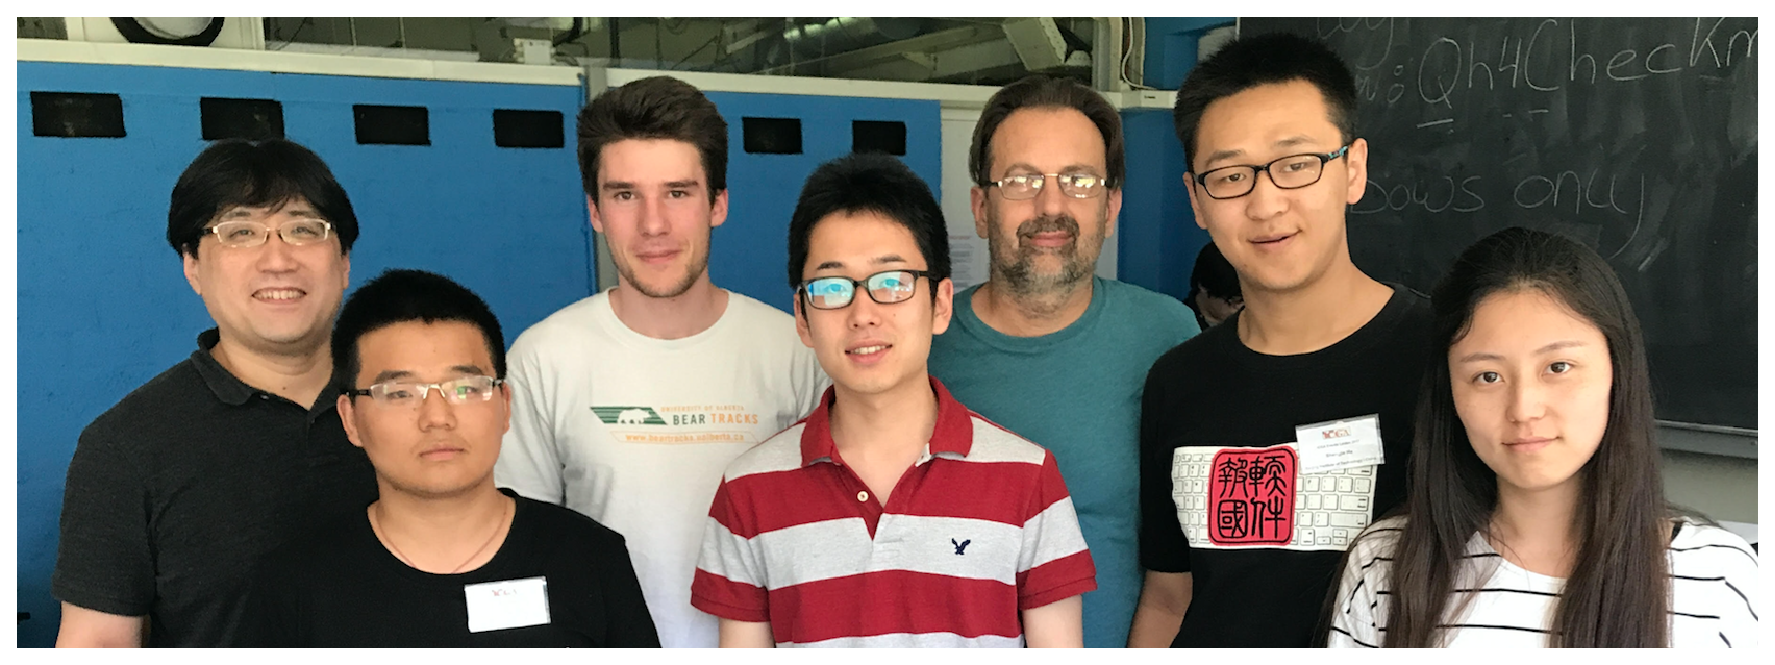
\includegraphics[width=\columnwidth]{photos/people-1.eps}\
\caption{Participants at the Hex competitions. From left,
Masahito Yamamoto, 
Wu Tong,
Noah Weninger, 
Kei Takada, 
Ryan Hayward, 
Ma Shengjie, 
Wu Tong (no relation to other Wu Tong).} \end{figure}

\section{The Tournaments}
There were two Hex tournaments at the 2017 Olympiad:
board size 11$\times$11 and board size 13$\times$13.
Three programs competed in each tournament.

The 11$\times$11 contestants were
\Hite{} by Ma Shengjie from China;
\Eo{} by Kei Takada, supervised by Masahito Yamamoto, from Japan;
and \Mx{}
by Broderick Arneson, Ryan Hayward, Philip Henderson, Aja Huang, 
Jakub Pawlewicz, Noah Weninger, and Kenny Young from Canada,
The 13$\times$13 contestants were
\Hent{} by Wu Tong from China;
\Eo{}; and
\Mc{} by Chao Gao from Canada.

\Mx{} \citebay{HAHMP13},
the winner of the previous seven Olympiad Hex competitions \citebay{HAHP13},
is an MCTS program that uses the Benzene Hex framework
built on the code base of \Fuego\ \citebay{fuego}.
%the Go program developed by Martin M\"{u}ller, Markus Enzenberger
%and others at the University of Alberta.
%Benzene allows virtual connection and
%inferior cell computations.
\Mx{} performs knowledge computation 
in UCT tree nodes visited at least 256 times.
\Mx{} ran on Firecreek, a 24 core shared-memory machine, 
with 4 cores reserved for the 
DFPNS solver \citebay{PawlH13}, which
produces perfect play if it solves the
position within the time allotted.
\Mx{} uses a book ---
built by Broderick Arneson with Thomas Lincke's method 
\citebay{DBLP:conf/cg/Lincke00}. 
Noah Weninger expanded the book and added a feature
allowing the use of rotational symmetry for openings
whose rotation is in the book.
For each board size, the book covers at least eight openings.

\Mc{} 
written top of \Mx{},
is a new version of MoHex with a convolutional neural policy net.
At each new node of the tree, the net biases child selection by
initializing child visit and win counts with artificial values.
\Mc{} ran remotely on a machine with 2 CPUs and 1 GPU.

\Eo{} is a stronger version of the program that competed in the 
2016 Olympiad.
\Eo{}, based on the Benzene framework, 
uses iterative deepening alpha-beta search 
with an evaluation function using a linear combination of
two network connectivity measures \citebay{TakadaHIY15}.
New this year, \Eo{} uses a convolutional neural policy network
for move ordering.
\Eo{} ran remotely on a machine
with two CPUs and one GPU,
with one CPU-thread for search and one CPU-thread for
Benzene's Depth-First Proof Number Search endgame solver.

\Hite{} and \Hent{} are new MCTS programs written 
respectively by Ma Shengjie and Wu Tong
of the Beijing Institute of Technology.
Each ran on a laptop.

Each tournament was scheduled for 8 games between
each two of the three competitors.
The tournaments started on July 1 and finished on July 5.
In most games, the losing operator resigned
soon after Benzene solved the game.

{\large\bf 11$\times$11 Tournament.}\footnote{Source files for this report, including .sgf files, at \url{https://github.com/ryanbhayward/icga-olympiad-hex}.}
The new program \Hite{} played strongly in the opening of
several of its games,
but without any virtual connection computation was unable
to win a game against \Eo{} or \Mx{}, which both
use Benzene's virtual connection engine and endgame solver.
For this reason, the operator chose to default its final games.

The contest for gold required a four-game playoff between
\Mx{}, whose code has not been changed in several years,
and \Eo{}, with a new policy net.
The result of the competition was not decided until the final game.

\hfill\begin{tabular}{|c|c|c|c|c|c|}
\hline 11x11 results &\Mx{} &\Eo{}  & \Hite{}  & total & result \\ 
\hline \Mx{}         &      &  7-5  &  3-0   & 10-5  &  gold \\
\hline \Eo{}         &  5-7 &       &  3-0   & 8-7   &  silver \\
\hline \Hite{}       &  0-3 &  0-3  &        & 0-6   &  bronze \\
\hline
\end{tabular}\hfill~

\iflong
This is the longer version, so we include all games.
\fi


%{\bf Game 1.}
%{\sc E-M 0-1.}
%1.B[a9] 2.W[b10] 3.B[f7] \ldots ~ ~ 
%
%{\bf Game 2.}
%{\sc M-H 1-0.}
%1.B[a2] 2.W[b9] 3.B[e7] \ldots ~ ~ 
%
%{\bf Game 3.}
%{\sc H-E 0-1.}
%1.B[a2] 2.W[swap] 3.B[g5] \ldots ~ ~ 
%
%{\bf Game 4.}
%{\sc M-E 1-0.}
%1.B[a6] 2.W[c9] 3.B[g7] \ldots ~ ~ 
%
%{\bf Game 5.}
%{\sc H-M 0-1.}
%1.B[a2] 2.W[g5] 3.B[f5] \ldots ~ ~ 
%
%{\bf Game 6.}
%{\sc E-H 1-0.}
%1.B[a2] 2.W[b9] 3.B[e7] \ldots ~ ~ 
%
%{\bf Game 7.}
%{\sc E-M 0-1.}
%1.B[k5] 2.W[e7] 3.B[g6] \ldots ~ ~ 
%
%{\bf Game 8.}
%{\sc M-H 1-0.}
%1.B[a7] 2.W[swap] 3.B[g5] \ldots ~ ~ 
%
%{\bf Game 9.}
%{\sc H-E 0-1.}
%1.B[a2] 2.W[swap] 3.B[j3] \ldots ~ ~ 
%
%{\bf Game 10.}
%{\sc M-E 1-0.}
%1.B[a6] 2.W[c9] 3.B[g7] \ldots ~ ~ 
%
%\begin{figure}[hbp]
%\includegraphics[scale=1.3]{games/pix/01-em-0-1.eps}\hspace*{-1cm}\
%\includegraphics[scale=1.3]{games/pix/01-em-completion.eps}\
%\caption{Game 1: \Eo-\Mx\ 0-1. Black resigned after move 34 (on left), when it saw the loss.}
%\end{figure}
%
%\begin{figure}[hbp]
%\includegraphics[scale=1.3]{games/pix/10-me-1-0.eps}\hspace*{-1cm}\
%\includegraphics[scale=1.3]{games/pix/10-me-completion.eps}
%\caption{Game 10: \Mx-\Eo\ 1-0. Black resigned after move 38 (on left), when it saw the loss.}
%\end{figure}

%\begin{figure}[hbp]
%\hspace*{-2.5cm}\
%\includegraphics[scale=1.3]{games/pix/01-em-0-1.eps}\hspace*{-2cm}\
%\includegraphics[scale=1.2]{games/pix/01-em-completion.eps}\hspace*{-2cm}\
%\includegraphics[scale=1.2]{games/pix/02-mh-1-0.eps}\hspace*{-2cm}\
%\includegraphics[scale=1.2]{games/pix/03-he-0-1.eps}
%\caption{Game 1: \Eo-\Mx\ 0-1. Game 2: \Mx-\Hz\ 1-0. Game 3: \Hz-\Eo\ 0-1.} 
%\end{figure}

%\begin{figure}[hbp]
%\hspace*{-2.5cm}\
%\includegraphics[scale=1.2]{games/pix/04-me-1-0.eps}\hspace*{-2cm}\
%\includegraphics[scale=1.2]{games/pix/05-hm-0-1.eps}\hspace*{-2cm}\
%\includegraphics[scale=1.2]{games/pix/06-eh-1-0.eps}
%\caption{Game 4: \Mx-\Eo\ 1-0. Game 5: \Hz-\Mx\ 0-1. Game 6: \Eo-\Hz\ 1-0.}
%\end{figure}
%
%\begin{figure}[hbp]
%\hspace*{-2cm}\
%\includegraphics[scale=1.2]{games/pix/07-em-0-1.eps}\hspace*{-2cm}\
%\includegraphics[scale=1.2]{games/pix/08-mh-1-0.eps}\hspace*{-2cm}\
%\includegraphics[scale=1.2]{games/pix/09-he-0-1.eps}
%\caption{Game 7: \Eo-\Mx\ 0-1. Game 8: \Mx-\Hz\ 1-0. Game 9: \Hz-\Eo\ 0-1.}
%\end{figure}

%\begin{figure}[hbp]
%\hspace*{-2cm}\
%\includegraphics[scale=1.3]{games/pix/10-me-1-0.eps}\hspace*{-2cm}\
%\includegraphics[scale=1.2]{games/pix/10-me-completion.eps}\hspace*{-2cm}\
%\includegraphics[scale=1.2]{games/pix/em-friendly-0-1.eps}\hspace*{-2cm}\
%\includegraphics[scale=1.2]{games/pix/me-friendly-0-1.eps}
%\caption{Game 10: \Mx-\Eo\ 1-0. Exhibition 1-thread games: \Eo-\Mx\ 0-1, \Mx-\Eo\ 0-1.}
%\end{figure}

~

{\large\bf 13$\times$13 Tournament.}

\hfill\begin{tabular}{|c|c|c|c|c|c|}
\hline 13x13 results &\Mc{} &\Eo{}  &\Hent{} & total & result \\ 
\hline \Mc{}         &      &  4-0  & 4-0  & 8-0   & gold \\
\hline \Eo{}         &  0-4 &       & 4-0  & 4-4   & silver \\
\hline \Hent{}         &  0-4 &  0-4  &      & 0-8   & bronze \\
\hline
\end{tabular}\hfill~

%{\bf Game 1.}
%{\sc E-M 0-1.}
%1.B[?] 2.W[?] 3.B[?] \ldots ~ ~ 
%
%{\bf Game 2.}
%{\sc M-H 1-0.}
%1.B[?] 2.W[?] 3.B[?] \ldots ~ ~ 
%
%{\bf Game 3.}
%{\sc H-E 0-1.}
%1.B[?] 2.W[?] 3.B[?] \ldots ~ ~ 
%
%{\bf Game 4.}
%{\sc M-E 1-0.}
%1.B[?] 2.W[?] 3.B[?] \ldots ~ ~ 
%
%{\bf Game 5.}
%{\sc H-M 0-1.}
%1.B[?] 2.W[?] 3.B[?] \ldots ~ ~ 
%
%{\bf Game 6.}
%{\sc E-H 1-0.}
%1.B[?] 2.W[?] 3.B[?] \ldots ~ ~ 
%
%{\bf Game 7.}
%{\sc E-M 0-1.}
%1.B[?] 2.W[?] 3.B[?] \ldots ~ ~ 
%
%{\bf Game 8.}
%{\sc M-H 1-0.}
%1.B[?] 2.W[?] 3.B[?] \ldots ~ ~ 
%
%{\bf Game 9.}
%{\sc H-E 0-1.}
%1.B[?] 2.W[?] 3.B[?] \ldots ~ ~ 
%
%{\bf Game 10.}
%{\sc M-E 1-0.}
%1.B[?] 2.W[?] 3.B[?] \ldots ~ ~ 
%
%{\bf Game 11.}
%{\sc H-M 0-1.}
%1.B[?] 2.W[?] 3.B[?] \ldots ~ ~ 
%
%{\bf Game 12.}
%{\sc E-H 1-0.}
%1.B[?] 2.W[?] 3.B[?] \ldots ~ ~ 

%\begin{figure}[hbp]
%\hspace*{-2cm}\
%\includegraphics[scale=1.1]{games/pix/13-01-em-0-1.eps}\hspace*{-2cm}\
%\includegraphics[scale=1.1]{games/pix/13-02-mh-1-0.eps}\hspace*{-2cm}\
%\includegraphics[scale=1.1]{games/pix/13-03-he-0-1.eps}
%\caption{Game 1: \Eo-\Mx\ 0-1. Game 2: \Mx-\Hz\ 1-0. Game 3: \Hz-\Eo\ 0-1.}
%\end{figure}

%\begin{figure}[hbp]
%\hspace*{-2cm}\
%\includegraphics[scale=1.1]{games/pix/13-04-me-1-0.eps}\hspace*{-2cm}\
%\includegraphics[scale=1.1]{games/pix/13-05-hm-0-1.eps}\hspace*{-2cm}\
%\includegraphics[scale=1.1]{games/pix/13-06-eh-1-0.eps}
%\caption{Game 4: \Mx-\Eo\ 1-0. Game 5: \Hz-\Mx\ 0-1. Game 6: \Eo-\Hz\ 1-0.}
%\end{figure}

%\begin{figure}[hbp]
%\hspace*{-2cm}\
%\includegraphics[scale=1.1]{games/pix/13-07-em-0-1.eps}\hspace*{-2cm}\
%\includegraphics[scale=1.1]{games/pix/13-08-mh-1-0.eps}\hspace*{-2cm}\
%\includegraphics[scale=1.1]{games/pix/13-09-he-0-1.eps}
%\caption{Game 7: \Eo-\Mx\ 0-1. Game 8: \Mx-\Hz\ 1-0. Game 9: \Hz-\Eo\ 0-1.}
%\end{figure}

%\begin{figure}[hbp]
%\hspace*{-2cm}\
%\includegraphics[scale=1.1]{games/pix/13-10-me-1-0.eps}\hspace*{-2cm}\
%\includegraphics[scale=1.1]{games/pix/13-11-hm-0-1.eps}\hspace*{-2cm}\
%\includegraphics[scale=1.1]{games/pix/13-12-eh-1-0.eps}
%\caption{Game 10: \Mx-\Eo\ 1-0. Game 11: \Hz-\Mx\ 0-1. Game 12: \Eo-\Hz\ 1-0.}
%\end{figure}

\section{Conclusions}
On 11$\times$11 \Mx\ and \Eo\ seem evenly matched.
\Mx{}'s search seems too narrow, especially near the opening.
In positions where there are several good options,
initial playout results often bias the final move selection,
with the result that \Mx\ can make bad moves early in the game.
This is the primary purpose of \Mx's book, to 
avoid bad early move selection,
and played a role in the final playoff game, where
\Eo{} opened at H2.

{\bf Acknowledgements.}
We thank the NSERC Discovery Grant Program for research funding and
Martin M\"{u}ller for the loan of his machine Firecreek.
\bibliography{rpt}
\end{document}
